\documentclass[sigconf]{acmart}

% DAI 2026 Research Track camera-ready metadata for the OpenReview archive.
% ACM publication identifiers and rights commands remain provisional until
% the conference publication stage supplies them.
\acmYear{2026}
\acmConference[DAI '26]
  {The Eighth International Conference on Distributed Artificial Intelligence}
  {November 29--December 2, 2026}
  {Hong Kong, China}
\acmBooktitle{The Eighth International Conference on Distributed Artificial
  Intelligence (DAI '26), November 29--December 2, 2026, Hong Kong, China}
\setcopyright{none}
\copyrightyear{}
\acmDOI{}
\acmISBN{}
\settopmatter{printacmref=true}

\usepackage{amsmath}
\usepackage{array}
\usepackage{booktabs}
\usepackage{graphicx}
\usepackage{tabularx}
\usepackage{xcolor}
\emergencystretch=1em

\newcommand{\method}{\textsc{SciRelay}}
\newcommand{\ndcg}{nDCG}

\title{SciRelay: Calibrated Bid-and-Relay for Communication-Bounded Scientific Evidence Retrieval}

\author{Wenbin Ma}
\affiliation{%
  \institution{Jiangnan University}
  \city{Wuxi}
  \country{China}}
\email{mwb060822@gmail.com}
\renewcommand{\shortauthors}{Wenbin Ma}

\begin{abstract}
Distributed retrieval agents may hold disjoint corpora and use heterogeneous scorers, making raw relevance scores incomparable. Sending every candidate defeats the communication boundary. We introduce \method, a training-free bid-and-relay protocol: each agent emits at most four 20-byte sketches containing a document fingerprint, rank-normalized position, and compact query-term coverage; a coordinator greedily maximizes a monotone submodular surrogate and relays at most $B$ documents. On 5,183 SciFact abstracts partitioned among 4--16 agents, \method{} improves \ndcg{} over the strongest decentralized baseline by 0.038--0.049 under lexical heterogeneity and 0.108--0.150 with one score-inflating agent. A held-out 809-query split confirms the six gains at 0.042--0.052 and 0.125--0.183. A frozen SPECTER extension confirms gains of 0.059--0.076 with dense agents and 0.164--0.223 when lexical and dense agents coexist. On the 505 confirmation claims with SUPPORT/CONTRADICT labels, relayed evidence raises a fixed FEVER-trained NLI verifier's accuracy by 1.2--3.8 points; only the fault-condition interval excludes zero. A 171,332-document TREC-COVID study reproduces fault robustness but leaves the smaller heterogeneity transfer uncertain. These results support a lightweight protocol contract, not universal superiority or Byzantine security. Code, pinned model revisions, per-query outputs, and executable claim checks accompany the submission.
\end{abstract}

\keywords{distributed AI, multi-agent retrieval, communication budget, federated search, submodular selection, scientific evidence}
\ccsdesc[500]{Computing methodologies~Multi-agent systems}
\ccsdesc[300]{Information systems~Information retrieval}

\begin{document}
\maketitle

\section{Introduction}

Multi-agent systems can distribute a large corpus across specialized or access-constrained agents, but distribution creates an information-selection bottleneck. A local agent may find useful evidence, yet a coordinator must decide which evidence deserves scarce communication before seeing full document content. This decision becomes fragile when agents use different retrievers or score scales, and adversarial or malfunctioning agents can report inflated scores. Relaying all candidates is robust but communication-inefficient; sorting incomparable raw scores is cheap but unreliable.

Figure~\ref{fig:overview} summarizes the studied boundary. Agents keep disjoint corpora and may use incompatible scorers. They first expose only fixed-width, score-free \emph{bid sketches}---the control-channel messages, called \emph{bids} below. The coordinator selects complementary bids and then admits at most $B$ full abstracts to downstream reasoning.

\begin{figure*}[t]
\centering
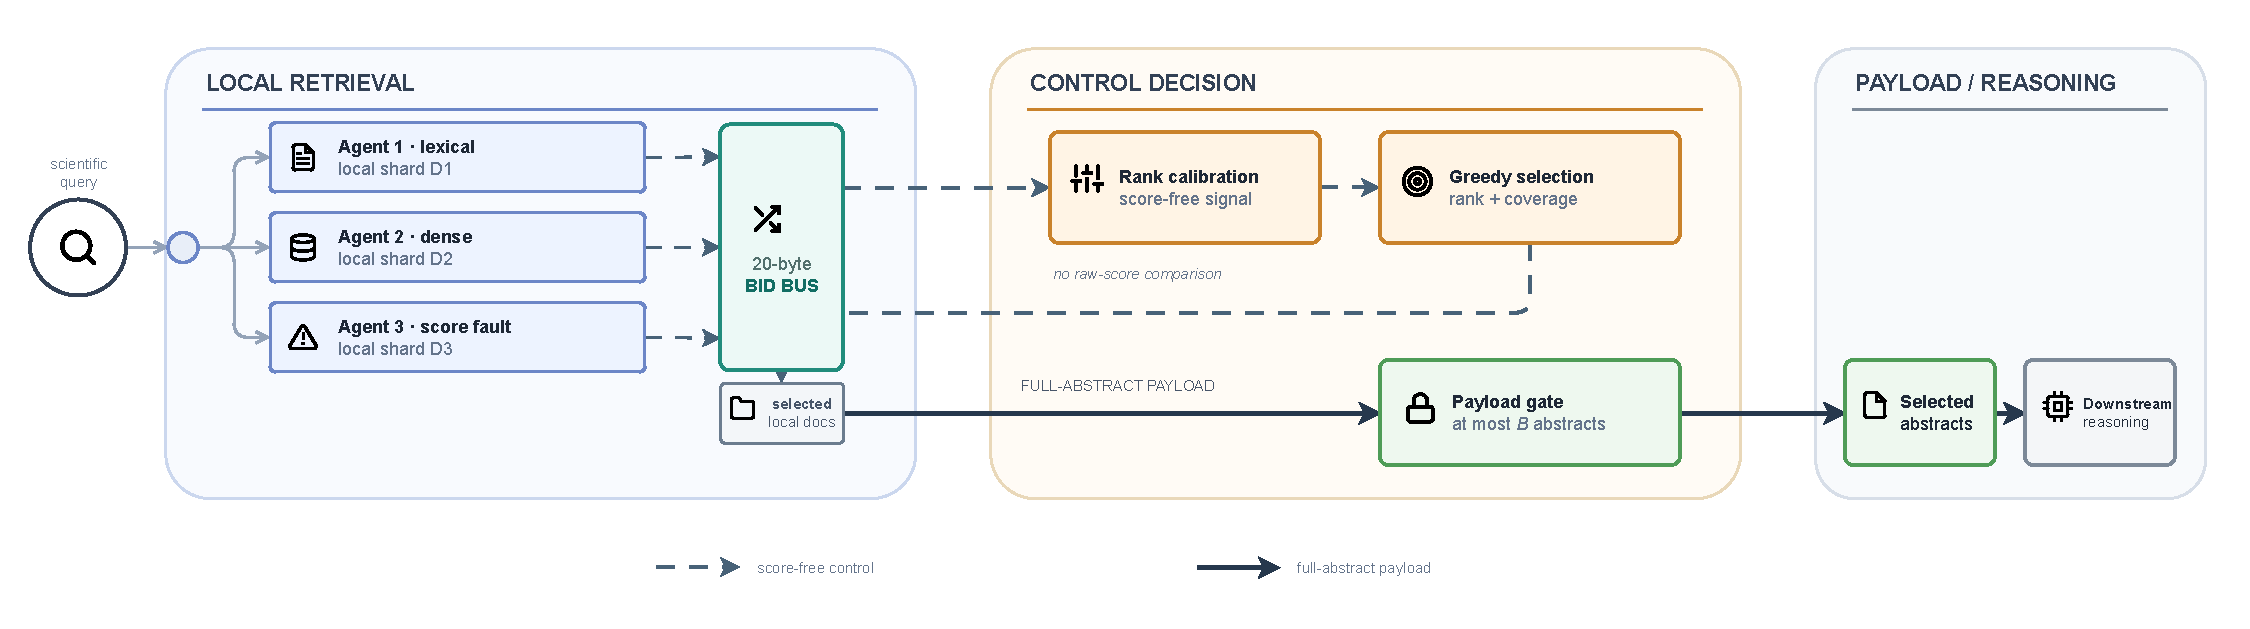
\includegraphics[width=\textwidth,trim=0 18 0 18,clip]{figures/scirelay_concept.pdf}
\caption{SciRelay's two-channel communication contract. A query is fanned to disjoint local shards; each agent emits a fixed-width, score-free bid sketch, and the coordinator selects complementary bids before requesting at most $B$ full abstracts for downstream reasoning. Thin gray arrows fan out the query, dashed arrows trace score-free control, and solid arrows denote full-abstract payloads.}
\Description{A left-to-right concept diagram separates local retrieval, control decisions, and downstream reasoning. A query fans out to three local agents, which feed fixed-width bid sketches to a bid bus. The coordinator calibrates rank, selects complementary bids, gates at most B payloads, and sends selected abstracts to downstream reasoning. Thin gray arrows show query fan-out, dashed arrows show score-free control, and solid arrows show full-abstract payloads.}
\label{fig:overview}
\end{figure*}

Recent work studies whether language-model agents can coordinate over information silos~\cite{zhang2026silobench}, how learned agents exchange messages~\cite{foerster2016communicate,das2019tarmac}, and how multi-agent topologies can be pruned or evolved to reduce tokens~\cite{wang2025agentdropout,tian2026queenbee}. These approaches largely ask \emph{who communicates with whom} or whether agents can reason after communication. We ask a complementary question: with a fixed star topology and a hard full-document budget, \emph{which content should be transmitted}? The question also connects to federated search, where resource selection and result merging must operate across distributed collections~\cite{shokouhi2011federated}.

The contribution is the protocol contract, not a new rank, coverage, or greedy component: each document has one owner, each agent emits only a fixed-width sketch, and the coordinator chooses payloads before seeing their content. This is an interface-level contribution for distributed AI systems: the contract makes the observable state, communication budget, failure surface, and admission decision independently auditable. Rank is the shared relevance signal and query-term coverage the shared content signal, combined under a hard payload budget to make score mismatch and integrity stress auditable.

We organize the study around four research questions. \textbf{RQ1} asks whether score-free, coverage-aware bids improve evidence selection when local score scales differ or one agent inflates scores, and whether they remain useful when scores are comparable. \textbf{RQ2} asks how the answer changes with relay budget, agent count, shard imbalance, and component removal. \textbf{RQ3} asks whether the frozen protocol transfers to a much larger biomedical collection. \textbf{RQ4} asks whether it survives dense candidate generation and changes a fixed downstream fact verifier. This framing separates supported conditions from universal superiority.

We propose \method, a compact two-stage protocol for distributed scientific evidence retrieval. First, every agent sends up to four bids. Each bid represents a local candidate using an agent-comparable rank statistic and a query-term bitmap rather than depending on an uncalibrated score. Second, the coordinator greedily selects a set of complementary bids and requests only those full documents. The selection objective is monotone submodular, so the standard greedy rule has a $(1-1/e)$ approximation guarantee under a cardinality budget~\cite{nemhauser1978submodular}.

Our contributions are:
\begin{itemize}
  \item We formulate bid selection as a communication-bounded bridge between local retrieval and downstream evidence use, explicitly separating compact bid sketches on the control channel from full-document payloads.
  \item We introduce a score-scale-robust, training-free protocol with a 20-byte bid model and a submodular objective combining calibrated local rank with complementary query coverage.
  \item We evaluate 4--16 agents, three relay budgets, heterogeneous retrieval, a score-inflating faulty agent, imbalanced shards, and a 171,332-document external corpus, with query-level inference and held-out confirmation.
  \item We add frozen SPECTER and FEVER-trained NLI evaluations, and preserve boundaries: lexical homogeneous gains are unreliable, cross-domain heterogeneity is uncertain, and downstream gains are statistically supported only under the declared fault.
\end{itemize}

\section{Related Work}

\paragraph{Information silos and multi-agent communication.}
Silo-Bench evaluates distributed computation when agents hold partial state and exposes a communication-reasoning gap~\cite{zhang2026silobench}. Learned communication methods such as differentiable inter-agent learning and targeted messaging optimize task-conditioned messages~\cite{foerster2016communicate,das2019tarmac}. AgentDropout removes redundant agents and edges~\cite{wang2025agentdropout}, while QueenBee Planner evolves communication topologies and skills~\cite{tian2026queenbee}. Reliability-Contagion analyzes how failures can propagate through LLM-agent networks~\cite{niu2026reliability}. In contrast, our topology, retrievers, and budget are fixed; the optimized object is the set of full evidence payloads. No policy learning, LLM inference, or paid API is required.

\paragraph{Federated retrieval and rank fusion.}
Federated search separates resource selection from result merging across searchable collections~\cite{shokouhi2011federated}. CORI estimates collection relevance from query-term collection statistics~\cite{callan1995distributed}, while ReDDE estimates relevant-document distributions using collection samples~\cite{si2003redde}. Those methods decide which resources to search and assume collection-level evidence unavailable in our contract: every shard is already queried, no sample or global term statistic crosses the boundary, and payload admission occurs from per-document sketches under a hard $B$. RRF instead avoids direct score comparability by aggregating ranks~\cite{cormack2009rrf}. Because each document has one owner, repeated votes are unavailable. We compare not only RRF and raw-score fusion but also local Min--Max and z-score normalization, isolating whether ordinary score calibration suffices before adding query-conditioned coverage.

\paragraph{Scientific retrieval and verification.}
SciFact introduced expert-written claims, evidence, and SUPPORT/CONTRADICT labels~\cite{wadden2020scifact}; BEIR provides standardized retrieval snapshots~\cite{thakur2021beir}. SPECTER learns citation-informed scientific document representations~\cite{cohan2020specter}. We use its pinned encoder for semantic candidate generation, then test whether selected abstracts affect a fixed DeBERTa-v3 NLI model trained on MNLI, FEVER, and ANLI rather than SciFact~\cite{he2021debertav3,williams2018mnli,thorne2018fever,nie2020anli}. Retrieval uses \ndcg{}~\cite{jarvelin2002ndcg}, recall, hit rate, and reciprocal rank; verification uses accuracy, balanced accuracy, and macro-F1.

\section{Problem Formulation}

Let a corpus $D$ be partitioned into disjoint shards $D_1,\ldots,D_N$, one per retrieval agent. For query $q$, agent $a$ can inspect only $D_a$ and returns at most $m$ compact bids. The coordinator may request at most $B$ full documents, where $B\in\{2,4,8\}$ in our study. A policy must map the union of bids to a set $A$ of distinct documents with $|A|\leq B$.

We account for communication as two channels. A bid sketch has fixed width $w$ bytes, while relaying document $d$ costs its UTF-8 payload size $\ell(d)$. Total query communication is
\begin{equation}
 C(A)=N m w+\sum_{d\in A}\ell(d).
\end{equation}
All compared decentralized methods see the same candidate limit $m$ and document budget $B$. Raw-score fusion uses a 12-byte bid model, local Min--Max/z-score fusion uses 10 bytes, RRF uses 9 bytes, and \method{} uses 20 bytes; payload cost is measured exactly from selected abstracts.

The design target is not to outperform an oracle. A centralized lexical retriever that indexes all documents is reported as a non-distributed reference. Our primary comparison is the strongest decentralized baseline within each scenario and budget.

\subsection{Protocol Contract and Failure Surface}

The coordinator operates in two stages. Before selection it may inspect only bid fields, not titles, abstracts, or relevance labels. After selection it requests at most $B$ payloads and preserves their greedy order as the returned ranking. Agent-to-coordinator channels are assumed to identify the sending agent, and the document fingerprint is used only for deduplication and payload verification. Documents are disjoint in our benchmark; nevertheless, deduplication makes the selection rule well-defined if replicas occur in a deployment.

The communication budget constrains full-document payloads rather than agent turns. Every agent emits at most $m$ bids in one control round, after which the coordinator makes one payload request. Thus all methods receive the same candidate pool and the same $B$; they differ only in how that pool is ordered. This isolates content selection from topology design, dialogue policy, and downstream answer generation.

Our faulty condition is deliberately narrow. One authenticated agent replaces its local top candidates with low-scoring local documents and reports synthetic raw scores from 1.2 to 0.9. The condition tests score-scale integrity, not identity spoofing, collusion, message omission, or adaptive manipulation of the term bitmap. \method{} does not infer trust scores and cannot certify that a bitmap is truthful before a payload arrives. A deployed system should bind fingerprints and masks to authenticated payloads and reject mismatches. These assumptions define the empirical claim boundary rather than a general Byzantine model.

\section{SciRelay}

\subsection{Compact Local Bids}

Agent $a$ ranks its local shard and emits its top $m=4$ candidates. For candidate $d$ at local rank $r\in\{1,\ldots,m\}$, the bid contains:
\begin{itemize}
  \item a 64-bit document fingerprint;
  \item the local rank and quantized lexical-coverage fraction;
  \item a 64-bit bitmap of query terms present in the document; and
  \item two bytes of origin/check metadata (the channel also identifies the agent).
\end{itemize}
The resulting model is 20 bytes per bid. The largest query in the snapshot has 28 distinct normalized terms, so one 64-bit bitmap is sufficient. Fingerprint collisions are not observed; a production system should resolve any collision before payload transfer.

Raw scores remain available only to raw-score baselines and a diagnostic ablation. We use ``calibrated'' only in the limited operational sense of normalizing a candidate's local position; no probabilistic calibration or cross-agent fitting is claimed. \method{} therefore uses rank-normalized local position
\begin{equation}
 \rho(b)=1-\frac{r(b)-1}{m},
\end{equation}
which is comparable across word and character retrievers without fitted calibration data.

\begin{figure}[t]
  \small
  \hrule
  \vspace{3pt}
  \textbf{Input:} bids $\mathcal{B}$, relay budget $B$, weights $\alpha,\beta,\gamma$.\\
  \textbf{State:} selected bids $A\leftarrow\varnothing$; covered query terms $U\leftarrow\varnothing$.
  \begin{enumerate}
    \setlength{\itemsep}{0pt}
    \setlength{\parskip}{0pt}
    \item Remove any bid whose fingerprint is already represented in $A$.
    \item For every remaining bid $b$, compute
    \[
      g(b\mid A)=\alpha\rho(b)+\beta c_b+
      \gamma |T_b\setminus U|/|T_q|.
    \]
    \item Add the bid with maximum $g(b\mid A)$; break an exact tie by document identifier and update $U\leftarrow U\cup T_b$.
    \item Repeat until $|A|=B$ or no distinct bid remains; request the selected payloads in greedy order.
  \end{enumerate}
  \vspace{-2pt}
  \hrule
  \caption{Deterministic coordinator-side selection. Raw retrieval scores never enter the final rule.}
  \Description{Pseudocode for greedy SciRelay selection from compact bids under a full-document budget.}
  \label{fig:protocol}
\end{figure}

\subsection{Submodular Relay Selection}

For bid $b$, let $T_b\subseteq T_q$ be its covered query terms and $c_b=|T_b|/|T_q|$. For a candidate set $A$, \method{} maximizes
\begin{align}
F(A)={}&\alpha\sum_{b\in A}\rho(b)+\beta\sum_{b\in A}c_b \\
 &+\gamma\frac{|\bigcup_{b\in A}T_b|}{|T_q|},
\end{align}
with nonnegative weights $(\alpha,\beta,\gamma)=(0.35,0.29,0.16)$. The first two terms are modular and the third is a coverage function, so their nonnegative sum is monotone submodular. Greedy marginal-gain selection under $|A|\leq B$ therefore attains at least $(1-1/e)$ of the optimum of this surrogate~\cite{nemhauser1978submodular}. This guarantee applies to $F$, not to relevance metrics.

\paragraph{Formal guarantee.}
For any fixed bid pool and nonnegative $(\alpha,\beta,\gamma)$, $F$ is monotone submodular; the deterministic greedy set satisfies $F(A_{\mathrm{g}})\geq(1-1/e)F(A^\star)$ under $|A|\leq B$. This is a guarantee for the declared sketch surrogate only, not for nDCG, recall, or answer quality.

The coordinator repeatedly adds the bid with largest marginal $F$ gain, breaking ties by document identifier, and requests the corresponding full payloads. Complexity is $O(BNm)$, at most 512 bid evaluations for the largest setting.

The coverage term has diminishing returns: for $X\subseteq Y$ and any bid $b\notin Y$, the newly covered set $T_b\setminus\bigcup_{x\in X}T_x$ contains the corresponding set under $Y$. Its normalized cardinality therefore has no smaller marginal gain for $X$. Adding the two modular terms preserves submodularity and monotonicity, establishing the greedy guarantee. The proof also exposes a boundary: the guarantee concerns the declared sketch fields and surrogate $F$; an agent that falsifies coverage can invalidate the intended semantics without violating the optimization calculation.

Three operational invariants make the implementation auditable. First, no fingerprint is selected twice. Second, selection uses no corpus-global statistic or qrel after local retrieval; calibrated rank depends only on the emitted list length. Third, document identifiers resolve exact ties, so reruns are deterministic for a fixed candidate pool. If $L_{\max}$ bounds a payload, the measured protocol obeys
\begin{equation}
 C(A)\leq Nmw+B L_{\max},
\end{equation}
and its control component is exactly $Nmw$. In the eight-agent setting this is $8\times4\times20=640$ bytes per query under the stated field-width model.

Initial development versions also used the local raw-score margin and a source-diversity reward. Development ablations showed that the former was harmful across heterogeneous scales and the latter was consistently neutral to slightly harmful for disjoint shards. Both were removed before the held-out confirmation and external-corpus runs. We retain them as ablations and record the revision in the artifact history.

\section{Experimental Design}

\subsection{Dataset and Splits}

We use the BEIR SciFact snapshot: 5,183 title-abstract documents, 1,109 queries, and binary evidence qrels~\cite{wadden2020scifact,thakur2021beir}. During development, 20 queries from the conventional test split were inspected for smoke testing. To avoid presenting a touched split as unseen, we designate all 300 conventional test queries as the \emph{development study}. The 809 conventional training queries are not used for method or weight selection and become a \emph{held-out confirmation split}. This reversal of conventional labels is explicit in configurations and per-query outputs; the split is not presented as a new benchmark test set.

Documents are assigned to agents by a stable seeded hash. Five seeds (11, 23, 47, 89, 131) are used in the development and scaling studies. The confirmation uses three previously unused seeds (173, 251, 419). No relevance labels enter retrieval, bidding, or selection.

\paragraph{Data preprocessing and split governance.}
The bundled snapshot stores one JSON line per document and query plus explicit train/test qrels. Only positive qrels are treated as relevant. The retrieval index concatenates title and abstract, lowercases text, and is fitted once on all 5,183 documents; it never observes qrels. Stable BLAKE2b hashing of \texttt{seed:document-id} assigns balanced shards. The imbalanced scenario instead samples owners from Zipf weights proportional to $i^{-1.2}$ using the shard seed. Query coverage uses distinct lowercase alphanumeric tokens longer than two characters, a deliberately simpler representation than the retrieval vectorizers.

The split reversal prevents an optimistic ``test'' label from hiding development contact. Method weights, component removal, and reporting choices were frozen using the 300-query development study. Only then were the 809 confirmation queries and their three shard seeds executed. The two studies are never pooled. The lexical main, scaling, ablation, and confirmation runs contain 144,000, 216,000, 64,800, and 116,496 policy records. The dense development and confirmation extensions add 81,000 and 131,058 records. All are retained in the artifact.

\paragraph{External-corpus protocol.}
After freezing the complete method on SciFact, we run the same eight-agent protocol on the BEIR TREC-COVID collection: 171,332 scientific documents, 50 topics, and pooled relevance judgments~\cite{voorhees2020treccovid,thakur2021beir}. We map every positive grade to binary relevance to match the SciFact metric implementation. The five development shard seeds, all four scenarios, $m=4$, the three budgets, retriever settings, and \method{} weights are reused without adjustment. Vectorizers are necessarily fitted on the new corpus, but no qrel enters indexing or selection. TREC-COVID therefore tests scale and domain transfer; its 50 topics make it a complementary external stress study, not a replacement for the larger SciFact confirmation.

\subsection{Retrievers, Scenarios, and Baselines}

Local retrieval uses deterministic TF-IDF~\cite{salton1988term}. Word agents use 1--2 word n-grams; character agents use 3--5 character n-grams. We evaluate:
\begin{description}
  \item[Homogeneous:] every agent uses the word retriever.
  \item[Heterogeneous:] even agents use word retrieval and odd agents use character retrieval.
  \item[Faulty:] the heterogeneous setting plus agent 0 selecting low-scoring local documents and reporting inflated raw scores.
  \item[Imbalanced:] heterogeneous retrievers with Zipf-weighted shard sizes.
\end{description}
The fault is intentionally synthetic and tests one concrete score-integrity failure, not Byzantine robustness in general. Because the injected agent changes both which local candidates are emitted and the raw scores attached to them, this experiment does not identify those two effects separately.

The frozen dense extension uses \texttt{allenai-specter} at revision \texttt{2c68eeca}. We L2-normalize final-layer [CLS] vectors, encode documents as title \texttt{[SEP]} abstract and queries as claim text, and use cosine similarity without relevance tuning. \emph{Dense homogeneous} assigns SPECTER to every agent; \emph{lexical--dense heterogeneous} alternates word TF-IDF and SPECTER; \emph{dense faulty} injects the same agent-0 corruption into dense retrieval. Candidate limit, shards, budgets, weights, lexical bid bitmap, policies, and query-level inference remain unchanged.

Baselines are random bid selection, round robin by local rank, raw-score sorting, local Min--Max and z-score normalization, and RRF~\cite{cormack2009rrf}. A centralized word TF-IDF retriever is a reference, not a feasible decentralized baseline. All policies receive identical local top-four candidate pools.

\paragraph{Baseline semantics and fairness.}
Raw-score sorting exposes score-scale failure. Local Min--Max and z-score fusion normalize the four emitted scores independently within each agent; Min--Max collapses to round robin when $B\leq N$ because every agent's top bid maps to one, whereas z-score also reflects local score dispersion. RRF assigns $1/(60+r)$ to each bid; with one owner per document it cannot accumulate votes. The ``best decentralized baseline'' is the maximum-mean member of raw score, local Min--Max, local z-score, RRF, and round robin; random is a seeded diagnostic and never wins. The centralized reference and \method{} do not participate. All raw records are retained, making comparator choice auditable.

The control-byte model counts policy-specific sketch fields: 20 bytes for \method{}, 12 for raw score, 10 for locally normalized scores, and 9 for RRF. Random and round robin are recorded as zero \emph{incremental feature} bytes because their ordering requires no feature beyond the common candidate envelope. The model omits framing, authentication, request headers, retransmission, and serialization overhead shared by all policies. Consequently, bytes check that \method{}'s bid sketch is small relative to relayed abstracts, not end-to-end throughput or literal zero-byte baselines. The primary budget $B$ counts documents rather than bytes; total-byte columns are reported separately and should not be read as equal-byte comparisons.

\paragraph{Fixed retrieval and method settings.}
Word TF-IDF uses 1--2 grams, English stop-word removal, sublinear term frequency, document frequency range $[2,0.98|D|]$, and at most 60,000 features. Character TF-IDF uses boundary-aware 3--5 grams, minimum document frequency 3, sublinear term frequency, and at most 50,000 features. We fix $m=4$, $B\in\{2,4,8\}$, and $(\alpha,\beta,\gamma)=(0.35,0.29,0.16)$ for all lexical and dense cells. A development-only guardrail varies $m\in\{2,4,8\}$ and each nonzero weight by $\pm20\%$ without changing the frozen protocol.

\subsection{Metrics and Inference}

The primary metric is \ndcg{} at relay budget $B$; we also report recall, hit rate, MRR, payload bytes, and control bytes. Headline tables retain the strongest decentralized baseline selected by cell mean as a descriptive, conservative comparator. To guard against comparator-selection uncertainty, sensitivity uses fixed references: RRF for heterogeneous and local z-score fusion for faulty scenarios. We first average each policy over shard seeds within query, then compute paired query-level differences. Intervals are percentile bootstrap 95\% confidence intervals with 10,000 resamples. Wilcoxon signed-rank tests are reported with Holm correction across the 12 development comparisons~\cite{holm1979procedure}; corrected tests are secondary because small positive effects need not be significant after family-wise correction.

The query, rather than a query-seed pair, is the inferential unit. Seed averaging prevents correlated shard realizations from being treated as independent relevance judgments. Bootstrap sampling uses a fixed seed of 20260810. The Wilcoxon test uses zero splitting; Holm correction is recomputed separately for the six confirmation and 12 external-corpus comparisons. The fixed-reference sensitivity analysis reports all comparator choices explicitly; the headline best-baseline intervals are labeled descriptive because they condition on the selected comparator and do not model selection uncertainty.

For downstream verification we use only the 505/809 confirmation claims carrying an unambiguous SUPPORT or CONTRADICT label; the other 304 are excluded before scoring. At $B=4$, the pinned \texttt{DeBERTa-v3-base-mnli-fever-anli} revision \texttt{6f5cf0a2} scores each relayed title--abstract as NLI premise and the claim as hypothesis. Within a relay set we take the document with the largest entailment-or-contradiction probability, then average its entailment-minus-contradiction margin across shard seeds. Comparators are fixed a priori by scenario: raw score for dense homogeneous and local z-score for lexical--dense and faulty. Accuracy differences use the same paired query bootstrap; the verifier is never trained or tuned on SciFact.

\subsection{Execution and Artifact Protocol}

Lexical experiments run on CPU with Python 3.12.4; their final Windows 11 runs required 171, 314, 68, and 226 seconds for SciFact main, scaling, ablation, and confirmation, plus 769 seconds for TREC-COVID. On an 8GB RTX 4060 Laptop GPU, pinned SPECTER encoding required 100 seconds, dense selection 16/19 seconds for development/confirmation, and 8,953 frozen NLI pairs 166 seconds. No paid API or remote inference is used; model identifiers, immutable revisions, preprocessing, and pair scores are recorded.

\textbf{Code availability.} The implementation, frozen configurations, per-query results, and executable claim checks are publicly available at \url{https://github.com/skmoca/SciRelay}. Each configuration writes raw per-query records, aggregates, paired comparisons, figures, and a run-information record. A separate verification entry point recomputes the submitted numeric claims from these records and verifies SHA-256 digests. The artifact includes a clean TREC-COVID download command rather than redistributing its 221 MB source file. Full clean-rerun and fast claim-check commands are separated so reviewers can inspect evidence without waiting for the largest index to rebuild.

\section{Results}

\begin{figure*}[t]
  \centering
  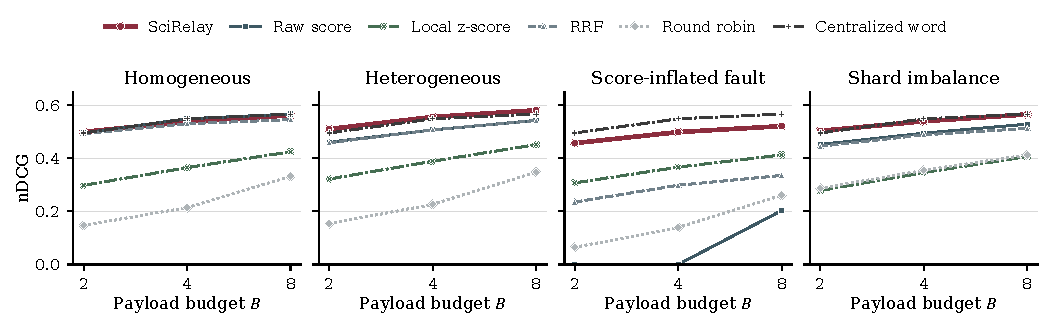
\includegraphics[width=0.98\textwidth]{../results/analysis/main_ndcg.pdf}
  \caption{Development \ndcg{} across full-document budgets and eight-agent scenarios. Centralized word retrieval is a non-distributed reference. Lines are means over 300 queries and five shard seeds.}
  \Description{Four line charts compare retrieval policies at relay budgets 2, 4, and 8 under homogeneous, heterogeneous, faulty-agent, and imbalanced scenarios. SciRelay is strongest among decentralized methods in the latter three scenarios and is close to raw-score fusion in the homogeneous scenario.}
  \label{fig:main}
\end{figure*}

\subsection{Development Results}

Figure~\ref{fig:main} and Table~\ref{tab:main} show the primary comparisons. In heterogeneous retrieval, \method{} gains 0.049, 0.048, and 0.038 \ndcg{} over the strongest decentralized baseline for budgets 2, 4, and 8. Under the score-inflating fault, local z-score fusion is stronger than RRF, yet \method{} retains gains of 0.150, 0.132, and 0.108. All six paired bootstrap intervals exclude zero. Holm-adjusted Wilcoxon values are not below 0.05 for the heterogeneous cells, so we do not claim corrected significance there; faulty-agent gains remain decisive.

\begin{table}[t]
\caption{Eight-agent development comparison. $\Delta$ is paired \ndcg{} gain over the strongest decentralized baseline; brackets are 95\% bootstrap CIs.}
\label{tab:main}
\small
\setlength{\tabcolsep}{3.2pt}
\begin{tabular}{llrrl}
\toprule
Scenario & $B$ & \method{} & Best base & $\Delta$ [95\% CI] \\
\midrule
Heterogeneous & 2 & .510 & .461 & .049 [.010,.089] \\
 & 4 & .556 & .508 & .048 [.018,.078] \\
 & 8 & .582 & .543 & .038 [.010,.067] \\
Faulty & 2 & .457 & .308 & .150 [.117,.182] \\
 & 4 & .499 & .367 & .132 [.107,.158] \\
 & 8 & .522 & .413 & .108 [.087,.130] \\
\bottomrule
\end{tabular}
\end{table}

The imbalanced setting also yields positive mean gains of 0.037--0.051, with bootstrap intervals above zero for all three budgets. In the homogeneous setting, differences from raw-score fusion range from $-0.010$ to $+0.004$, and every interval crosses zero (Table~\ref{tab:boundary}). This supports the intended boundary: calibrated bidding is useful when score scales or agent reliability differ, but it should not replace directly comparable scores by default. Failure to exclude zero is not evidence that the two methods are equivalent; it only prevents a reliable superiority claim.

\begin{table}[t]
\caption{Development boundary conditions. $\Delta$ is \method{} minus raw-score fusion; brackets are paired 95\% bootstrap CIs.}
\label{tab:boundary}
\small
\setlength{\tabcolsep}{4.2pt}
\begin{tabular}{llrrl}
\toprule
Scenario & $B$ & \method{} & Raw & $\Delta$ [95\% CI] \\
\midrule
Homogeneous & 2 & .500 & .496 & .004 [$-.034$,.042] \\
 & 4 & .539 & .549 & $-.010$ [$-.038$,.018] \\
 & 8 & .562 & .567 & $-.005$ [$-.029$,.020] \\
Imbalanced & 2 & .504 & .452 & .051 [.018,.086] \\
 & 4 & .540 & .495 & .045 [.016,.075] \\
 & 8 & .566 & .529 & .037 [.012,.063] \\
\bottomrule
\end{tabular}
\end{table}

At the middle budget, the nDCG pattern is accompanied by recall, hit-rate, and reciprocal-rank changes (Table~\ref{tab:secondary}). Heterogeneous \method{} improves recall from .592 to .641 and MRR from .490 to .537. Against local z-score fusion under the fault, recall rises from .473 to .577 and MRR from .339 to .482, so the gain is not a single-metric artifact. Conversely, the homogeneous row shows the expected small loss across recall and nDCG.

\begin{table}[t]
\caption{Secondary development metrics at $B=4$. ``Base'' is the strongest decentralized nDCG baseline in the cell.}
\label{tab:secondary}
\scriptsize
\setlength{\tabcolsep}{2.4pt}
\begin{tabular}{llrrrr}
\toprule
Scenario & Policy & Recall & Hit & MRR & \ndcg{} \\
\midrule
Homogeneous & \method{} & .620 & .637 & .521 & .539 \\
 & Base (Raw) & .651 & .667 & .523 & .549 \\
Heterogeneous & \method{} & .641 & .662 & .537 & .556 \\
 & Base (RRF) & .592 & .615 & .490 & .508 \\
Faulty & \method{} & .577 & .599 & .482 & .499 \\
 & Base (z-score) & .473 & .494 & .339 & .367 \\
Imbalanced & \method{} & .617 & .635 & .522 & .540 \\
 & Base (Raw) & .577 & .602 & .478 & .495 \\
\bottomrule
\end{tabular}
\end{table}

Across the main study, bid sketches equal 8.9\% of relayed payload bytes in aggregate. Figure~\ref{fig:communication} makes the amortization explicit: the control width stays fixed at 640 bytes per eight-agent query, while the payload grows with the relay budget. The added control cost buys score-scale robustness; it does not reduce the fixed number of full documents, which is held constant by design.

\begin{figure}[t]
  \centering
  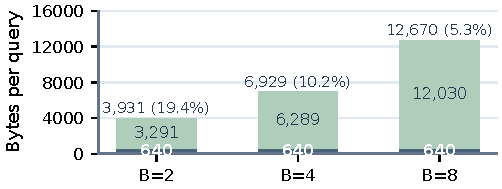
\includegraphics[width=\columnwidth]{figures/communication_breakdown.pdf}
  \caption{\method{} communication breakdown averaged across four development scenarios. Dark and pale segments denote fixed 640-byte control and mean full-abstract payload; labels report total bytes and the control/payload ratio.}
  \Description{Three stacked bars for relay budgets two, four, and eight. Each bar has an identical dark control segment of 640 bytes and a larger pale payload segment; total bytes and control-to-payload ratios are annotated above the bars.}
  \label{fig:communication}
\end{figure}

\subsection{Scale, Ablation, and Confirmation}

Scaling separates two effects. Under the faulty-agent stress test, \method{} beats the strongest decentralized baseline for every budget at 4, 8, and 16 agents; gains span 0.069--0.220 and every bootstrap interval excludes zero. Heterogeneous gains are also positive at every scale. At four agents they are 0.041--0.069 with intervals excluding zero, and at eight agents they are 0.038--0.049 with intervals excluding zero. At 16 agents the mean gains shrink to 0.025--0.029 and all three intervals cross zero. Thus score-fault robustness remains stable with scale, while the smaller heterogeneity benefit becomes uncertain as each local shard shrinks.

\begin{table*}[t]
\caption{Development scaling. Cells show \ndcg{} gain over the strongest decentralized baseline with paired 95\% bootstrap CI.}
\label{tab:scaling}
\centering
\small
\setlength{\tabcolsep}{7pt}
\begin{tabular}{llccc}
\toprule
Scenario & Agents & $B=2$ & $B=4$ & $B=8$ \\
\midrule
Heterogeneous & 4  & .069 [.037,.102] & .049 [.027,.071] & .041 [.022,.061] \\
 & 8  & .049 [.010,.089] & .048 [.018,.078] & .038 [.010,.067] \\
 & 16 & .029 [$-.013$,.071] & .029 [$-.004$,.063] & .025 [$-.005$,.055] \\
Faulty & 4  & .099 [.077,.122] & .074 [.058,.090] & .069 [.055,.083] \\
 & 8  & .150 [.117,.182] & .132 [.107,.158] & .108 [.087,.130] \\
 & 16 & .220 [.184,.258] & .197 [.167,.228] & .183 [.155,.210] \\
\bottomrule
\end{tabular}
\end{table*}

Table~\ref{tab:scaling} makes the distinction visible. Increasing the agent count reduces local shard size and changes which documents enter each top-four pool. The heterogeneous benefit is therefore candidate-limited at 16 agents: calibrated merging cannot recover relevant documents that fail to enter any bid list. The faulty-agent effect remains large because the dominant error is instead ranking corruption after candidates are formed.

\paragraph{Sensitivity guardrails.}
On development data only, perturbing each of $(\alpha,\beta,\gamma)$ individually by $\pm20\%$ leaves the $B=4$ gain at 0.062--0.069 for heterogeneous retrieval and 0.131--0.138 for faulty retrieval against fixed RRF and z-score references; every interval lower bound remains above 0.028 and 0.104, respectively. The full $m\times B$ grid for $m,B\in\{2,4,8\}$ also keeps all 18 target intervals above zero. At $B=4$, heterogeneous gains are 0.058--0.067 and faulty gains 0.100--0.279, while bid-control cost grows from 320 to 1,280 bytes as $m$ increases. A 16-agent probe yields heterogeneous gains of 0.039--0.043. These are stability diagnostics, not confirmation or post-hoc retuning; the frozen $m=4$ weights remain unchanged.

The final ablation averages the six heterogeneous/faulty budget cells. Removing rank calibration lowers \ndcg{} by 0.044 on average (cell range 0.034--0.054); removing both per-document and set-level query coverage lowers it by 0.261 (0.201--0.304). Re-introducing the discarded raw-score margin lowers it by 0.007, and adding source diversity lowers it by 0.002. These results support both retained components and the development-time simplification. They are not treated as independent confirmation because they were used to freeze the method. The joint coverage removal does not isolate set-level coverage from the simpler per-document lexical-match signal.

\begin{table}[t]
\caption{Ablation loss relative to final \method{}, averaged over six heterogeneous/faulty development cells. Every cell-level drop is positive.}
\label{tab:ablation}
\small
\setlength{\tabcolsep}{4pt}
\begin{tabular}{lrrr}
\toprule
Variant & Mean & Min & Max \\
\midrule
No query coverage & .261 & .201 & .304 \\
No rank calibration & .044 & .034 & .054 \\
Add raw margin & .007 & .005 & .009 \\
Add source diversity & .002 & .001 & .004 \\
\bottomrule
\end{tabular}
\end{table}

Coverage is the largest component because local lexical candidates often share a high-scoring query fragment. The set-level term rewards a bid that adds a missing fragment, while the per-document coverage term prevents a low-rank bid with one novel token from dominating. Rank calibration contributes less in absolute terms but is essential for cross-retriever comparability. The two rejected terms illustrate why more features need not help: a raw margin reintroduces the scale dependence the method is designed to avoid, and a source reward spends capacity on agent identity even when disjoint-shard evidence from one agent is complementary.

Finally, the held-out 809-query confirmation split reproduces the target effect with three new shard seeds. Heterogeneous gains are 0.052, 0.046, and 0.042 for budgets 2, 4, and 8; faulty-agent gains over local z-score fusion are 0.183, 0.142, and 0.125. All six paired 95\% intervals exclude zero, and all Holm-adjusted Wilcoxon values are below 0.001. The confirmation is reported separately from development and no \method{} weight or component was changed after reading it.

\begin{table}[t]
\caption{Held-out 809-query confirmation split. $\Delta$ is paired \ndcg{} gain over the listed best baseline.}
\label{tab:confirmation}
\scriptsize
\setlength{\tabcolsep}{2.6pt}
\begin{tabular}{llrrl}
\toprule
Scenario & $B$/Base & \method{} & Base & $\Delta$ [95\% CI] \\
\midrule
Heterogeneous & 2/Raw & .510 & .458 & .052 [.030,.073] \\
 & 4/Raw & .547 & .500 & .046 [.029,.065] \\
 & 8/Raw & .572 & .531 & .042 [.026,.058] \\
Faulty & 2/z-score & .453 & .270 & .183 [.161,.205] \\
 & 4/z-score & .484 & .342 & .142 [.125,.159] \\
 & 8/z-score & .508 & .383 & .125 [.111,.139] \\
\bottomrule
\end{tabular}
\end{table}

The heterogeneous confirmation effect is numerically close to development despite using 2.7 times as many queries and entirely new shard seeds. Faulty-agent gains are likewise stable. Corrected $p$-values are $<0.001$ in all six cells, but effect sizes and intervals remain the primary evidence: significance alone would not describe the homogeneous boundary or the practical gap under score inflation.

\subsection{Dense Retrieval and Downstream Verification}

Table~\ref{tab:dense-downstream} answers RQ4 with the original method and weights unchanged. On development, every dense-cell interval is positive: gains are 0.077--0.111 for dense homogeneous, 0.167--0.242 for lexical--dense heterogeneity, and 0.197--0.270 under the dense fault. The 809-query confirmation reproduces all nine signs and intervals. The lexical bitmap therefore remains useful when candidate generation is semantic: it supplies an exact query-conditioned signal complementary to SPECTER rank. This result revises, rather than hides, the lexical homogeneous boundary---common TF-IDF scores did not benefit reliably, whereas a common dense scorer plus a complementary lexical sketch does.

\begin{table*}[t]
\caption{Frozen SciFact dense extension and downstream closure. Retrieval cells are confirmation $\Delta$ nDCG with paired 95\% CIs against the fixed comparator. NLI reports $B=4$ accuracy for \method{}/comparator and paired difference over 505 labeled confirmation claims.}
\label{tab:dense-downstream}
\centering
\scriptsize
\setlength{\tabcolsep}{4.0pt}
\begin{tabular}{llcccl}
\toprule
Scenario & Comparator & $B=2$ & $B=4$ & $B=8$ & NLI accuracy; $\Delta$ [95\% CI] \\
\midrule
Dense homogeneous & Raw & .076 [.051,.100] & .069 [.049,.089] & .059 [.042,.076] & .808/.796; .012 [$-.014$,.038] \\
Lexical--dense & z-score & .223 [.199,.247] & .197 [.177,.216] & .164 [.148,.180] & .798/.774; .024 [$-.004$,.053] \\
Dense faulty & z-score & .239 [.217,.261] & .200 [.183,.219] & .177 [.162,.192] & .798/.760; .038 [.010,.065] \\
\bottomrule
\end{tabular}
\end{table*}

The NLI verifier reaches 0.836 accuracy (0.803 balanced accuracy) when given gold evidence, establishing that it is informative on this label subset. \method{} increases evidence hit rate at $B=4$ from 0.721 to 0.793 for dense homogeneous, 0.589 to 0.782 for lexical--dense, and 0.512 to 0.702 under fault. Accuracy moves in the same direction, but the first two intervals cross zero; only the 3.8-point fault gain is supported. Thus retrieval improvement is necessary but not sufficient for a downstream claim: the closed loop is decisive only under the declared integrity stressor.

\subsection{Frozen-Parameter External Corpus Study}

Table~\ref{tab:external} answers RQ3. On TREC-COVID, all six target mean differences remain positive. The heterogeneous gaps are 0.021--0.075, but their intervals cross zero because the collection has only 50 topics; transfer of the modest heterogeneity effect is therefore directionally consistent but statistically inconclusive. By contrast, the score-inflating fault produces gains of 0.087--0.140 over local z-score fusion, with all interval lower bounds above 0.06 and Holm-adjusted $p<0.001$. This reproduces the robustness finding on a corpus 33 times larger than SciFact without changing \method{}.

\begin{table}[t]
\caption{Frozen-parameter TREC-COVID study (171,332 documents, 50 topics, five seeds). $\Delta$ is paired \ndcg{} gain over the listed strongest decentralized baseline.}
\label{tab:external}
\scriptsize
\setlength{\tabcolsep}{2.6pt}
\begin{tabular}{llrrl}
\toprule
Scenario & $B$/Base & \method{} & Base & $\Delta$ [95\% CI] \\
\midrule
Heterogeneous & 2/Raw & .521 & .446 & .075 [$-.002$,.152] \\
 & 4/Raw & .487 & .430 & .057 [$-.006$,.119] \\
 & 8/Raw & .437 & .416 & .021 [$-.022$,.063] \\
Faulty & 2/z-score & .530 & .390 & .140 [.086,.194] \\
 & 4/z-score & .486 & .382 & .104 [.067,.141] \\
 & 8/z-score & .430 & .343 & .087 [.061,.114] \\
\bottomrule
\end{tabular}
\end{table}

TREC-COVID homogeneous gains are 0.047--0.101 with unadjusted intervals excluding zero, but no Holm-adjusted test is below 0.05; imbalanced gains are 0.015--0.085 and are supported only at $B=2$. These additional cells, retained in the artifact, reinforce the distinction between effect direction and family-wise evidence rather than establish universal complementarity.

\subsection{Query-Level Mechanism Analysis}

At $B=4$, the development fault gain is broad against z-score: \method{} wins on 175 queries, loses on 59, and has median $\Delta=0.099$. Under lexical heterogeneity it wins/ties/loses on 111/112/77 queries, so the positive mean coexists with a zero median. Lexical homogeneous losses outnumber wins (74 vs. 62). The paired query distributions are shown in Figure~\ref{fig:query-delta} in Appendix~C: the fault distribution is shifted positive, while the other scenarios retain substantial mass at zero. These counts support a conditional mechanism rather than a few-query explanation.

\section{Discussion}

\subsection{When Calibrated Relay Is Appropriate}

The results suggest a conditional deployment rule. If agents share both a scorer and its content signal, raw-score fusion is simpler unless validation supports the sketch: homogeneous word TF-IDF shows no reliable SciFact gain. A shared scorer alone is insufficient to decide; dense homogeneous agents benefit because the lexical bitmap supplies a complementary signal absent from SPECTER cosine rank. Deployments should therefore test signal complementarity, not infer it from scorer identity.

Calibrated relay is attractive when score comparability or integrity breaks. Local rank removes the scale difference between word and character TF-IDF, while coverage supplies a shared query-conditioned signal. Under the injected fault, raw scores are misleading; even per-agent z-score normalization preserves the faulty agent's fabricated local order, whereas coverage adds a content check. SciRelay is therefore a conservative bridge across a known interface mismatch, not a replacement for central ranking.

Budget and scale must be chosen together. At $B=2$, mistakes are costly; at $B=8$, control amortizes and relative gaps narrow. Increasing $N$ with $m=4$ shrinks local shards, and the 16-agent result shows no monotonic heterogeneous benefit. Deployments should monitor candidate recall and increase $m$ or merge tiny shards before refining the objective.

\subsection{Implications for LLM-Agent Systems}

The dense and NLI extensions instantiate \method{} as an evidence-selection layer before model reasoning. Pinned encoders, deterministic bid fields, and saved pair scores separate retrieval communication from prompt or model drift. The lexical--dense result shows that a cheap symbolic sketch can complement semantic candidates without transmitting embeddings. The NLI result also warns against equating evidence nDCG with answer quality: hit-rate gains are large in all three dense scenarios, yet only the fault condition yields a supported accuracy gain. An LLM deployment should therefore evaluate final answers and calibration rather than inherit the retrieval claim.

\subsection{From Stress Test to Robust Protocol}

The fault result motivates verification, not a security label. A deployment can authenticate senders, bind fingerprints to payloads, recompute masks, and log mismatches, but these checks cannot recover an unbid document. We do not test Sybils, collusion, omission, adaptive bitmap deception, or payload substitution; identity diversity was not protective in ablation. The evidence supports one score-integrity stressor, not Byzantine security.

\section{Limitations, Risks, and Scope}

The evidence covers two English collections; SciFact is compact and TREC-COVID has only 50 pooled topics. Dense evidence uses one SPECTER checkpoint and claim-to-document cosine setup, not modern instruction-tuned or domain-specialized retrievers. TREC-COVID grades are binarized. Multilingual or long-document corpora, graded objectives, and paraphrastic evidence remain untested; the lexical bitmap may under-reward semantically relevant documents with little word overlap.

Downstream evaluation covers 505 labeled claims and one FEVER-trained NLI checkpoint. The gold-evidence pilot reaches 0.836 accuracy but inspects the same labels, so the closure is exploratory rather than independent confirmation; selected abstracts may contain irrelevant sentences. This is not evidence about free-form LLM answers or scientific reasoning generally.

The local top-four pool is a hard bottleneck: at 16 agents, smaller shards alter candidate competition and heterogeneous intervals include zero because a coordinator cannot select unbid evidence. Adaptive bid limits and joint control/payload budgets are outside the frozen protocol; the centralized reference is not an upper bound, and the guarantee concerns only the surrogate.

The faulty-agent condition is one fixed score-integrity stress pattern, not security against adaptive Byzantine behavior, collusion, Sybils, omission, collisions, or deceptive bitmaps. Authentication and post-transfer checks are recommendations, not security experiments. The 20-byte bid is a field-width model; omitted framing and network effects preclude latency, bandwidth, energy, or throughput claims.

Weights and components were selected on 300 development queries; confirmation and TREC-COVID reduce but cannot eliminate corpus overfitting, and best-baseline intervals condition on observed comparator selection. We emphasize effect sizes, boundaries, and separate confirmation. Public abstracts and qrels involve no human subjects, personal data, paid model calls, or autonomous action.

\section{Conclusion}

\method{} uses compact, rank-calibrated bids to select evidence without comparing heterogeneous raw scores. SciFact development and confirmation support lexical heterogeneity and score-fault gains; frozen SPECTER extends the test to semantic candidates, while TREC-COVID leaves smaller cross-domain heterogeneity uncertain. A fixed NLI verifier supports a downstream gain under fault but not smaller gains otherwise. Together with the homogeneous negative result, this defines a conditional protocol rather than universal superiority.

\clearpage
\balance
\bibliographystyle{ACM-Reference-Format}
\bibliography{references}

\clearpage
\appendix
\raggedbottom

\section{Reproduction Contract}

The artifact exposes two levels of checking. A fast verifier loads the submitted per-query and paired-comparison files, checks the numeric ranges quoted in the paper, and validates the archive checksum manifest. A full rerun rebuilds retrieval indices and regenerates every result. After installing the pinned environment with \texttt{pip install -e .}, the principal commands are:

\begin{small}
\begin{verbatim}
python -m pytest -q
python scripts/verify_research_claims.py
python scripts/run_all_research.py
python scripts/encode_specter.py
python scripts/run_dense_research.py --config
  configs/dense_development.yaml
python scripts/run_dense_research.py --config
  configs/dense_confirmation.yaml
python scripts/run_nli_downstream.py
\end{verbatim}
\end{small}

The SciFact snapshot is bundled with its source notices. TREC-COVID, SPECTER weights, and NLI weights are intentionally omitted; scripts retrieve pinned public revisions. All result tables retain query, seed, scenario, budget, and policy identifiers. The NLI runner can reuse submitted pair scores for fast checking or recompute all 8,953 pairs.

\section{Bid Field Accounting}

The 20-byte bid is a field-width model, not a claim about a particular serializer. Figure~\ref{fig:bid-layout} makes the byte allocation explicit: eight bytes go to a document fingerprint, two bytes jointly to local rank and quantized per-document coverage, eight bytes to the query-term bitmap, and two bytes to origin/check metadata. The authenticated channel also identifies the sender. Common framing, payload requests, retransmission, and cryptographic authentication are outside the count; Figure~\ref{fig:communication} therefore reports an explicit analytical contract rather than measured network traffic.

\begin{figure}[ht]
  \centering
  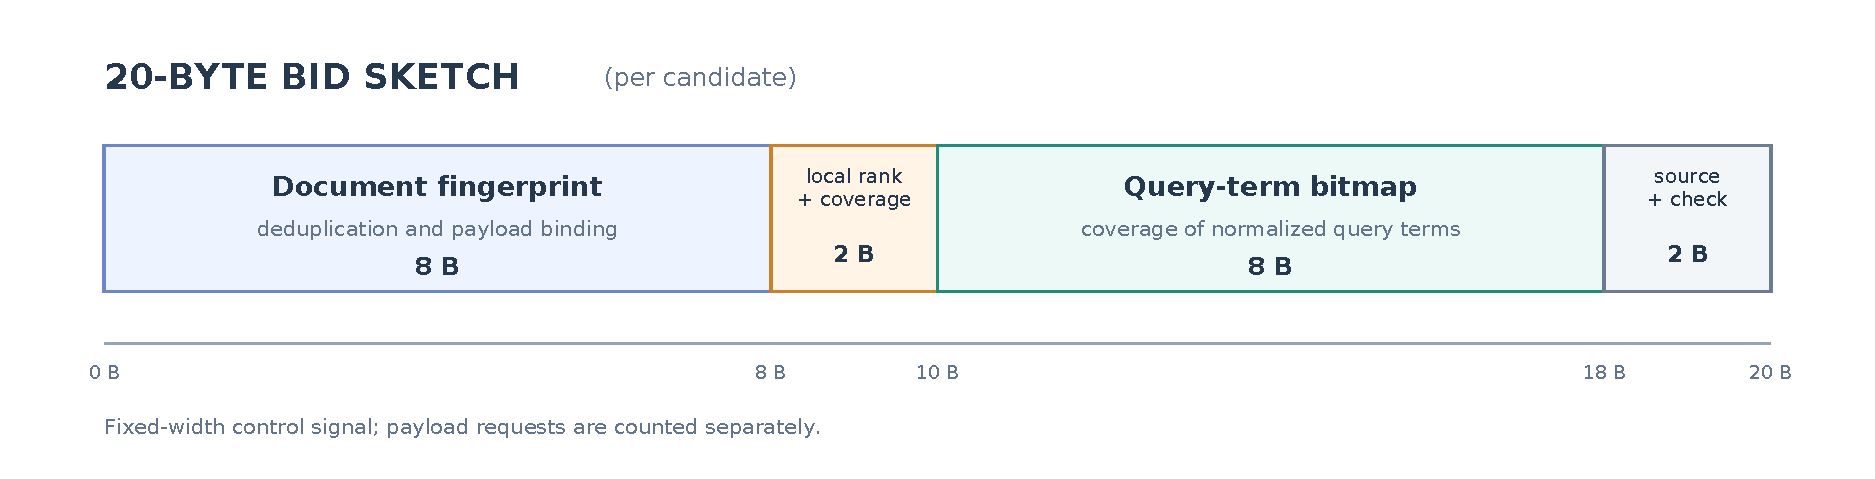
\includegraphics[width=\columnwidth]{figures/bid_field_layout.pdf}
  \caption{Fixed-width SciRelay bid layout for one candidate. Segment widths are proportional to the 20-byte field model; the authenticated channel's sender identity is represented by the source metadata field.}
  \Description{A horizontal 20-byte protocol layout divided into four proportional segments: an eight-byte document fingerprint, two bytes for local rank and coverage, an eight-byte query-term bitmap, and two bytes for source and check metadata.}
  \label{fig:bid-layout}
\end{figure}

\section{Control--Quality Guardrail}

Table~\ref{tab:bid-guardrail} promotes the development-only bid-limit probe to an explicit communication trade-off. Each cell uses three development shard seeds and the fixed $B=4$ comparator. Moving from $m=2$ to $m=4$ improves both SciRelay columns, while doubling control again to $m=8$ changes SciRelay nDCG by less than 0.001. The smaller faulty gain at larger $m$ reflects a stronger z-score comparator, not collapse of SciRelay. This diagnostic supports $m=4$ as an empirical knee for the studied eight-agent setting; it was not used to retune confirmation, dense, or external-corpus runs.

\begin{table}[ht]
\caption{Development-only control--quality guardrail at $N=8$ and $B=4$. Parentheses are gains over the fixed reference named in the header.}
\label{tab:bid-guardrail}
\centering
\scriptsize
\setlength{\tabcolsep}{4.0pt}
\begin{tabular}{rrrr}
\toprule
$m$ & Control bytes & Heterogeneous (RRF) & Faulty (z-score) \\
\midrule
2 & 320   & .551 (+.058) & .492 (+.279) \\
4 & 640   & .560 (+.067) & .502 (+.135) \\
8 & 1,280 & .560 (+.067) & .501 (+.100) \\
\bottomrule
\end{tabular}
\end{table}

\begin{figure}[ht]
  \centering
  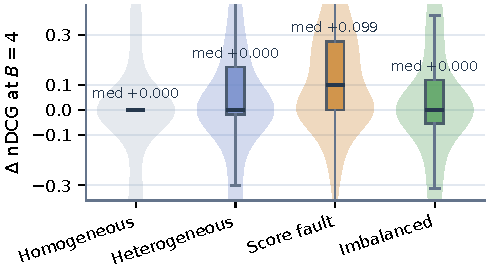
\includegraphics[width=\columnwidth]{figures/query_delta_distribution.pdf}
  \caption{Query-level $\Delta$ nDCG at $B=4$ over 300 development queries (means over shard seeds). Violins show distributions, boxes show interquartile ranges, and dark lines mark medians; labels report the medians.}
  \Description{Four colored violin and box distributions compare SciRelay with the strongest decentralized baseline. The faulty distribution is shifted upward with median plus 0.099, while homogeneous, heterogeneous, and imbalanced distributions have medians at zero and wider tails around zero.}
  \label{fig:query-delta}
\end{figure}

\end{document}
